\documentclass{article}

\usepackage{lmodern}
\usepackage{hyperref}
\usepackage{amsmath}
\usepackage{amssymb}
\usepackage[T1]{fontenc}
\usepackage{fancyhdr}
\usepackage{color,graphicx}
\pagestyle{fancy}
\lhead{Anirudhan J. Rajagopalan --- ajr619}

\begin{document}

\title{Kernel Based Approaches for Change-Point Detection --- Report 1}
\date{February 18, 2016}
\author{Anirudhan J. Rajagopalan, ajr619}

\maketitle

\newpage
\section{Offline Detection}
\subsection{Univariate Detection}
Lets assume a time series of observations $x_{1}, x_{2}, \ldots, x_{n} $ of independent random variables with parameters $(\mu_{1}, \sigma_{1}^{2}), (\mu_{2}, \sigma_{2}^{2}), \ldots, (\mu_{n}, \sigma_{n}^{2}) $.
Also lets assume that each of the observation $ x_{i} $ is normally distributed with mean $ \mu $ and common variance $\sigma^{2} \forall i \in 1, 2, \ldots ,n $.
When there is no change in mean, the hypothesis of stability (null hypothesis) is defined as
\begin{align}
  H_{0} : \mu_{1} = \mu_{2} = \cdots =  \mu_{n} = \mu
\end{align}
Lets suppose that there is a change in the mean in the observations at an unknown point $ K $.  This can be define dy
\begin{align}
  H_{1} : \mu_{1} = \ldots \mu_{k} \ne \mu_{k+1} \ldots =  \mu_{n}
\end{align}
In our experiments we are going to assume that we know $\mu_{1}, \mu_{n} $ and $ \sigma $ are known beforehand (Refer $2.1.1$ of~\cite{birkhauser_pscpa}).

\subsubsection{Experiments}
Finding the likelihood directly using the likelihood function is not practical as it is not computationally tractable for even a small value of n (600 in our case).  So we follow the steps given in the reference\cite{birkhauser_pscpa} to find the change point.

The offline changepoint detection problem, gives a pretty accurate value for changepoint at k = 300.  The different plots are as displayed below.

\begin{figure}[ht!]
  \centering
  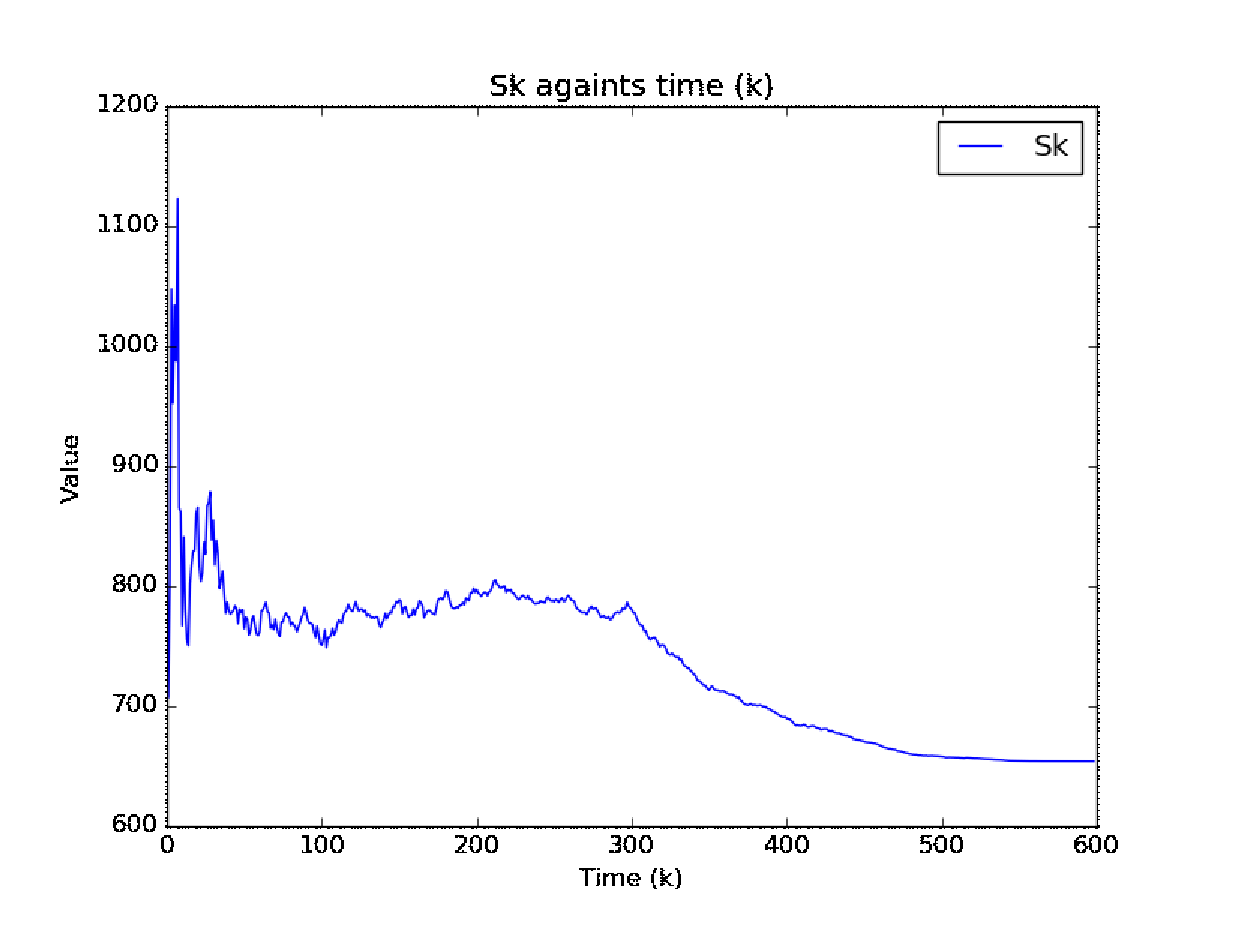
\includegraphics[width=0.75\textwidth]{images/1d_offline/sk}
  \caption{SK values for one dimensional offline detection problem.\label{fig:1d_sk}}
\end{figure}

\begin{figure}[ht!]
  \centering
  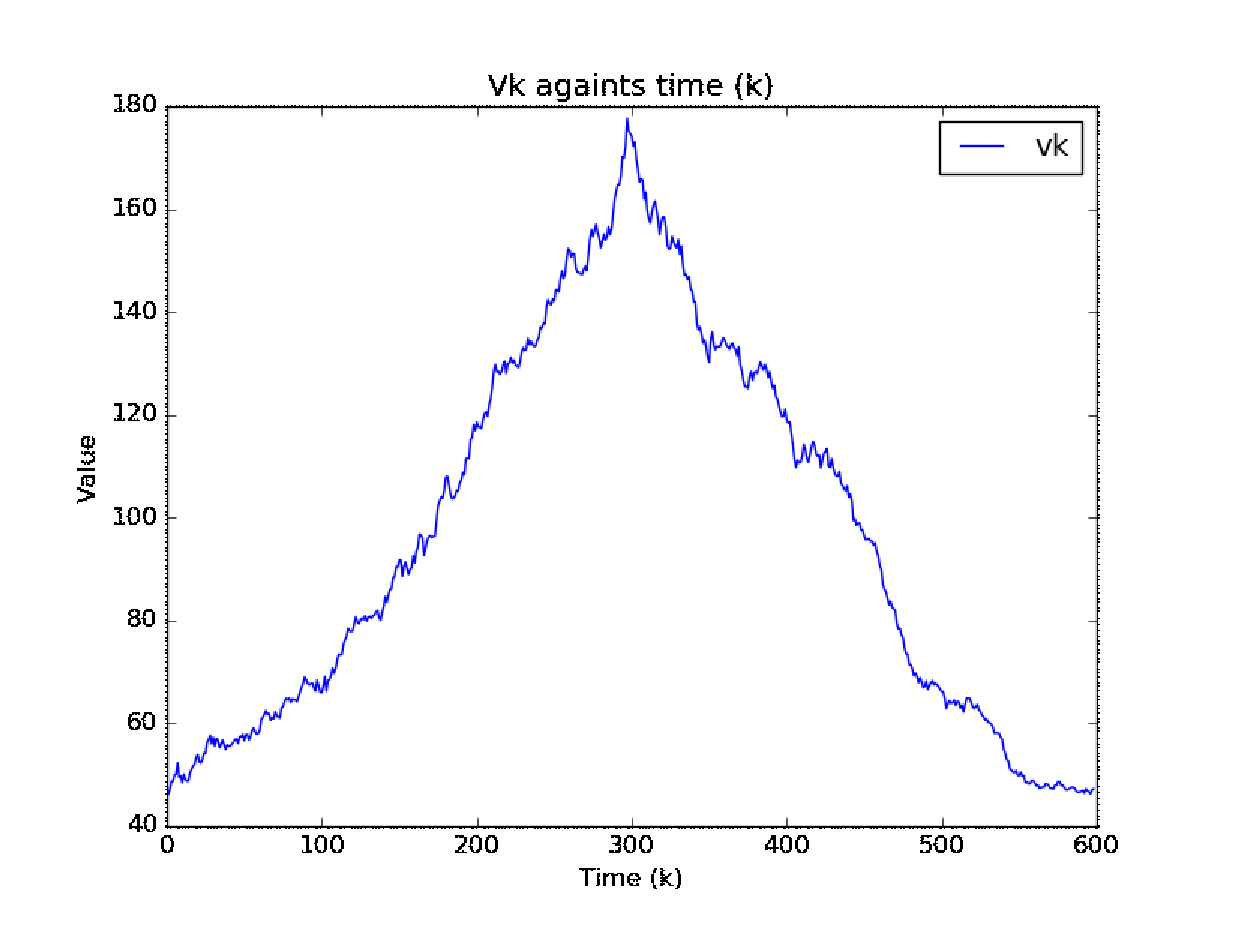
\includegraphics[width=0.75\textwidth]{images/1d_offline/vk}
  \caption{VK values for one dimensional offline detection problem.\label{fig:1d_vk}}
\end{figure}

\subsection{Multi-variate Detection}
\section{Online Detection}

\bibliographystyle{plain}
\bibliography{references}

\end{document}
